\documentclass[12pt]{article}

\usepackage[margin=1in]{geometry}

\usepackage{amsmath, graphicx, caption, subcaption, xcolor}

\graphicspath{{res/}}

\title{Gaseous Mass in the Galactic Plane}

\author{Lukas Finkbeiner}

% We probably want a basic run-down of a .fits file, but perhaps some of that can go in the introduction.

% Explain \alpha and \beta in the first figure.

\begin{document}

\maketitle

\begin{abstract}

% remember to motivate the paper

We study

1. velocity patterns of various H clouds using Doppler shifts

2. black hole mass

3. accuracy of a spiral arm fit

results, uncertainties.

\end{abstract}

\section{Introduction and Background}
% currently we need more connecting text and MORE MOTIVATION

Given certain patterns, how well does a spiral fit? We need to control for the total number of data. We want the normalization of any two compared sets to be the same (so, we scale accordingly). What numpy functions I used.

\begin{equation} \label{eq:spiral}
R_\text{arm} = R_0 e^{\kappa(\phi - \phi_0)}
\end{equation}

To explore these questions, we want to be able to examine the Doppler velocities and brightness temperatures associated with different parts of the galactic plane of the Milky Way. We want to examine power spectra collected for values of the galactic longitude $\ell$ on the range $-10^\circ$ to $250^\circ$. We will provide a more comprehensive analysis of our particular setup in the methods section. For now, we consider, in the abstract, two equations for calibrating the spectra. 

\begin{equation} \label{eq:line_shape}
T_\text{line} = G \, \frac{s_\text{on}}{s_\text{off}}
\end{equation}

\begin{equation} \label{eq:line_gain}
G = \frac{T_\text{sys, cal} - T_\text{sys, cold}}{\sum{(s_\text{cal} - s_\text{cold})}} \sum{s_\text{cold}}
\end{equation}

The first equation will be used to demonstrate a consistent HI signal by combining spectra for two different frequencies in the local oscillator. The second equation will be used to scale the power spectrum so that the y-axis carries information about the brightness temperatures associated with different frequencies on our spectra.

The following equation is a conclusion of the tangent-point method ($0^\circ < \ell \leq 90^\circ$) for converting galactic rotation to Doppler velocity (G.L. Verschuur and K. I. Kellermann, 1983). $V(R_\odot) \approx 220 $ km / s and $R_\odot \approx 8.5$ kpc $\equiv 2.6 \times 10^{17}$ km. 

\begin{equation} \label{eq:vel_dopp}
V_\text{Dopp} = \left[ \frac{V(R)}{R} - \frac{V(R_\odot)}{R_\odot} \right] R_\odot \sin(\ell)
\end{equation}

%\begin{equation}
%\frac{V_\text{Dopp}}{R_\odot \sin \ell} = \frac{V(R)}{R} - \frac{V(R_\odot)}{R_\odot}
%\end{equation}

%\begin{equation}
%\frac{V_\text{Dopp}}{R_\odot \sin \ell} + \frac{V(R_\odot)}{R_\odot} = \frac{V(R)}{R} = \frac{1}{R_\odot} \left[ \frac{V_\text{Dopp}}{\sin \ell} - V(R_\odot) \right] 
%\end{equation}

The following representation will be used in establishing the velocity curve inside the solar circle:

\begin{equation} \label{eq:vel_curve}
V(R) = \frac{R}{R_\odot} \left[ \frac{V_\text{Dopp}}{\sin \ell} - V(R_\odot) \right] 
\end{equation}

%This next form will be used in placing points outside the solar circle, to evaluate the spiral shape:

%\begin{equation}
%\frac{V_\text{Dopp}}{R_\odot \sin \ell} = \frac{V(R)}{R} - \frac{V(R_\odot)}{R_\odot}
%\end{equation}

%\begin{equation}
%\frac{V(R)}{R} = \frac{V_\text{Dopp}}{R_\odot \sin \ell} + \frac{V(R_\odot)}{R_\odot} 
%\end{equation}

%\begin{equation} \label{eq:outer_spiral}
%R = V(R) \left[ \frac{V_\text{Dopp}}{R_\odot \sin \ell} + \frac{V(R_\odot)}{R_\odot} \right]^{-1}
%\end{equation}

In preparation for our mass estimations, we start with the conventional

\begin{equation}
v^2 = \frac{G M_\text{gravitational}}{R} 
\end{equation}

Then, we re-arrange to get the desired form:

\begin{equation} \label{eq:mass}
M_\text{gravitational} = \frac{R v^2}{G} 
\end{equation}

As we collect Doppler velocities for each galactic longitude $\ell$, it is important to distinguish between $\ell$ and the radial distance $R$ of a hydrogen cloud to the galactic center. To estimate mass for the part of the galaxy inside the solar circle, we use the tangent point method by applying equation \ref{eq:vel_curve} with $R = R_\text{min} = R_\odot \sin \ell$. In figure \ref{fig:ell_vs_r}, we illustrate the range of radii associated with an arbitrary $\ell$. The tangent-point method necessarily excludes these other radii. Later on, in the observations section, we will visualize some consequences of this.

\begin{figure}
	\centering
	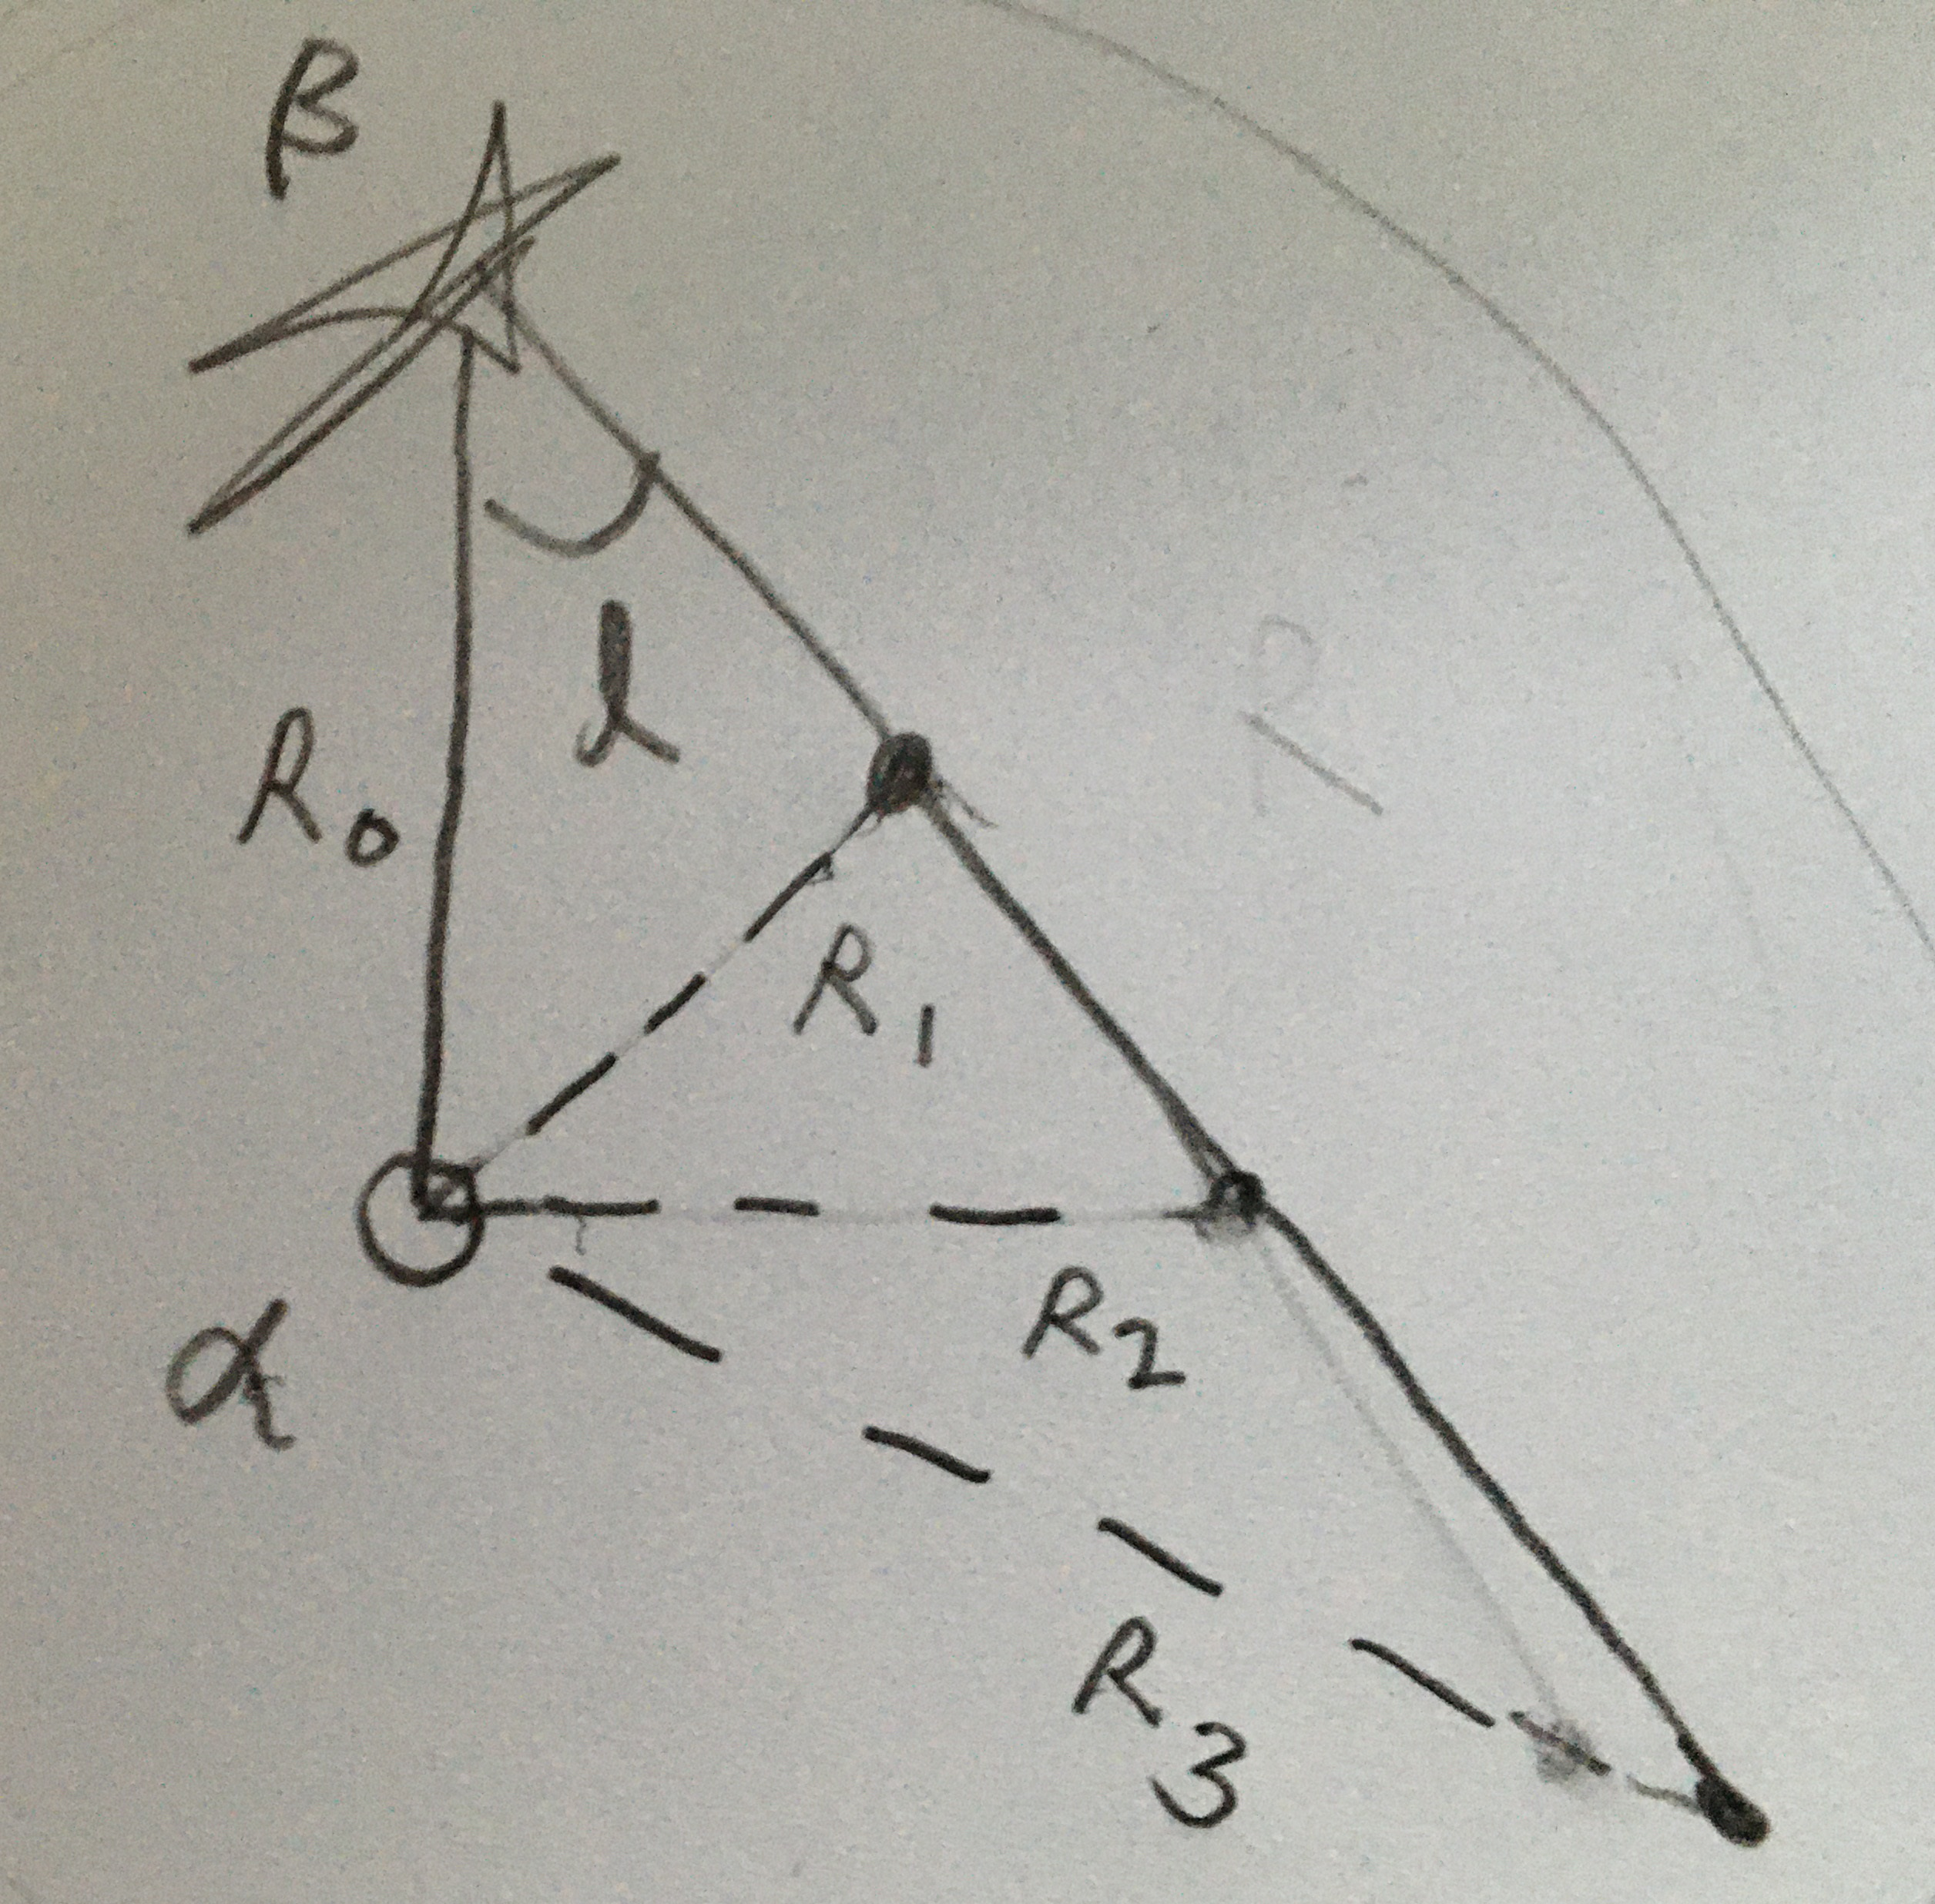
\includegraphics[width=.4\linewidth]{ell_versus_r}
	\caption{This is a simple illustration demonstrating how the value of $\ell$ can place constraints on valid values for $R$ (specifically, $R_2$ here represents the right-triangle case, for which the radius is minimized). However, since our universal value for galactic latitude $b = 0^\circ$ has no relevance to radial distances, no pair of galactic coordinates will specify the radius at which we are working. Consequently, the tangent-point method must explicitly establish that we work with a specific radius $R = R_\text{min}$.}
	\label{fig:ell_vs_r}
\end{figure}

\section{Methods}

\quad \quad To conduct all of our measurements of the galactic plane of the Milky Way, we run a tracking script on a remote computer linked to the Leuschner dish. Our full observation consists of 260 galactic coordinate pairs where the galactic latitude is a constant $0^\circ$ and the galactic longitude begins at $-9^\circ$ and increases in $1^\circ$ increments. We convert from galactic to topocentric coordinates using the same rotation matrices from lab 2 (Finkbeiner, 2020). We schedule our measurements by entering a value for the local sidereal time and considering which galactic coordinate pairs correspond to topocentric coordinate pairs which are currently accessible by the Leuschner dish (see figure \ref{fig:vis_demo} for an example case).

\begin{figure}
	\centering
	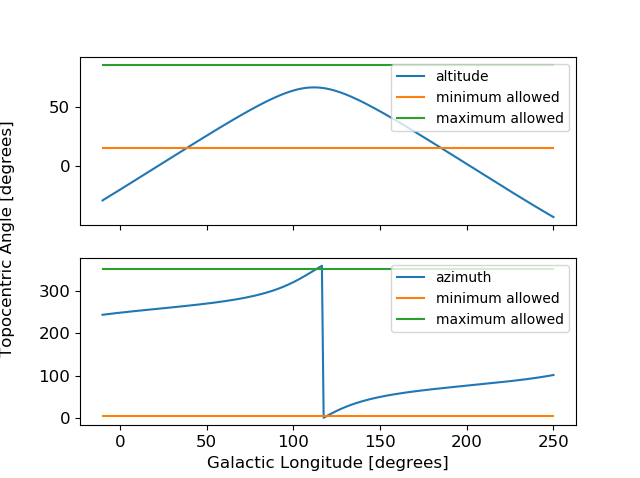
\includegraphics[width=.75\linewidth]{1940_10_05_2020}
	\caption{This is a visibility demonstration to clarify our observation process: we hold the local sidereal time fixed and plot the topocentric coordinate conversions for all values of the galactic longitude $\ell$ on our range. We began this project with the nominal range of $\ell \in [-10^\circ, 250^\circ]$. By calculating similar visibility curves for a full sidereal day, we are able to classify some of our observations with higher risk for obstruction (particularly when the target altitude is close to the dish's minimum attainable altitude). We also calculated that $\ell=-10^\circ$ is not visible for any sufficiently wide segment of the day. This visibility plot was generated at 19:40 on the tenth of May.}
	\label{fig:vis_demo}
\end{figure}

As a demonstration of the Leuschner dish signal chain (illustrated in figure \ref{fig:sig_chain}), we show how we map a set of input signals to a final frequency axis for our plots (frequency versus brightness temperature). Since we are considering only frequency, this allows us to skip over the amplifiers and attenuators.

\begin{figure}
	\centering
	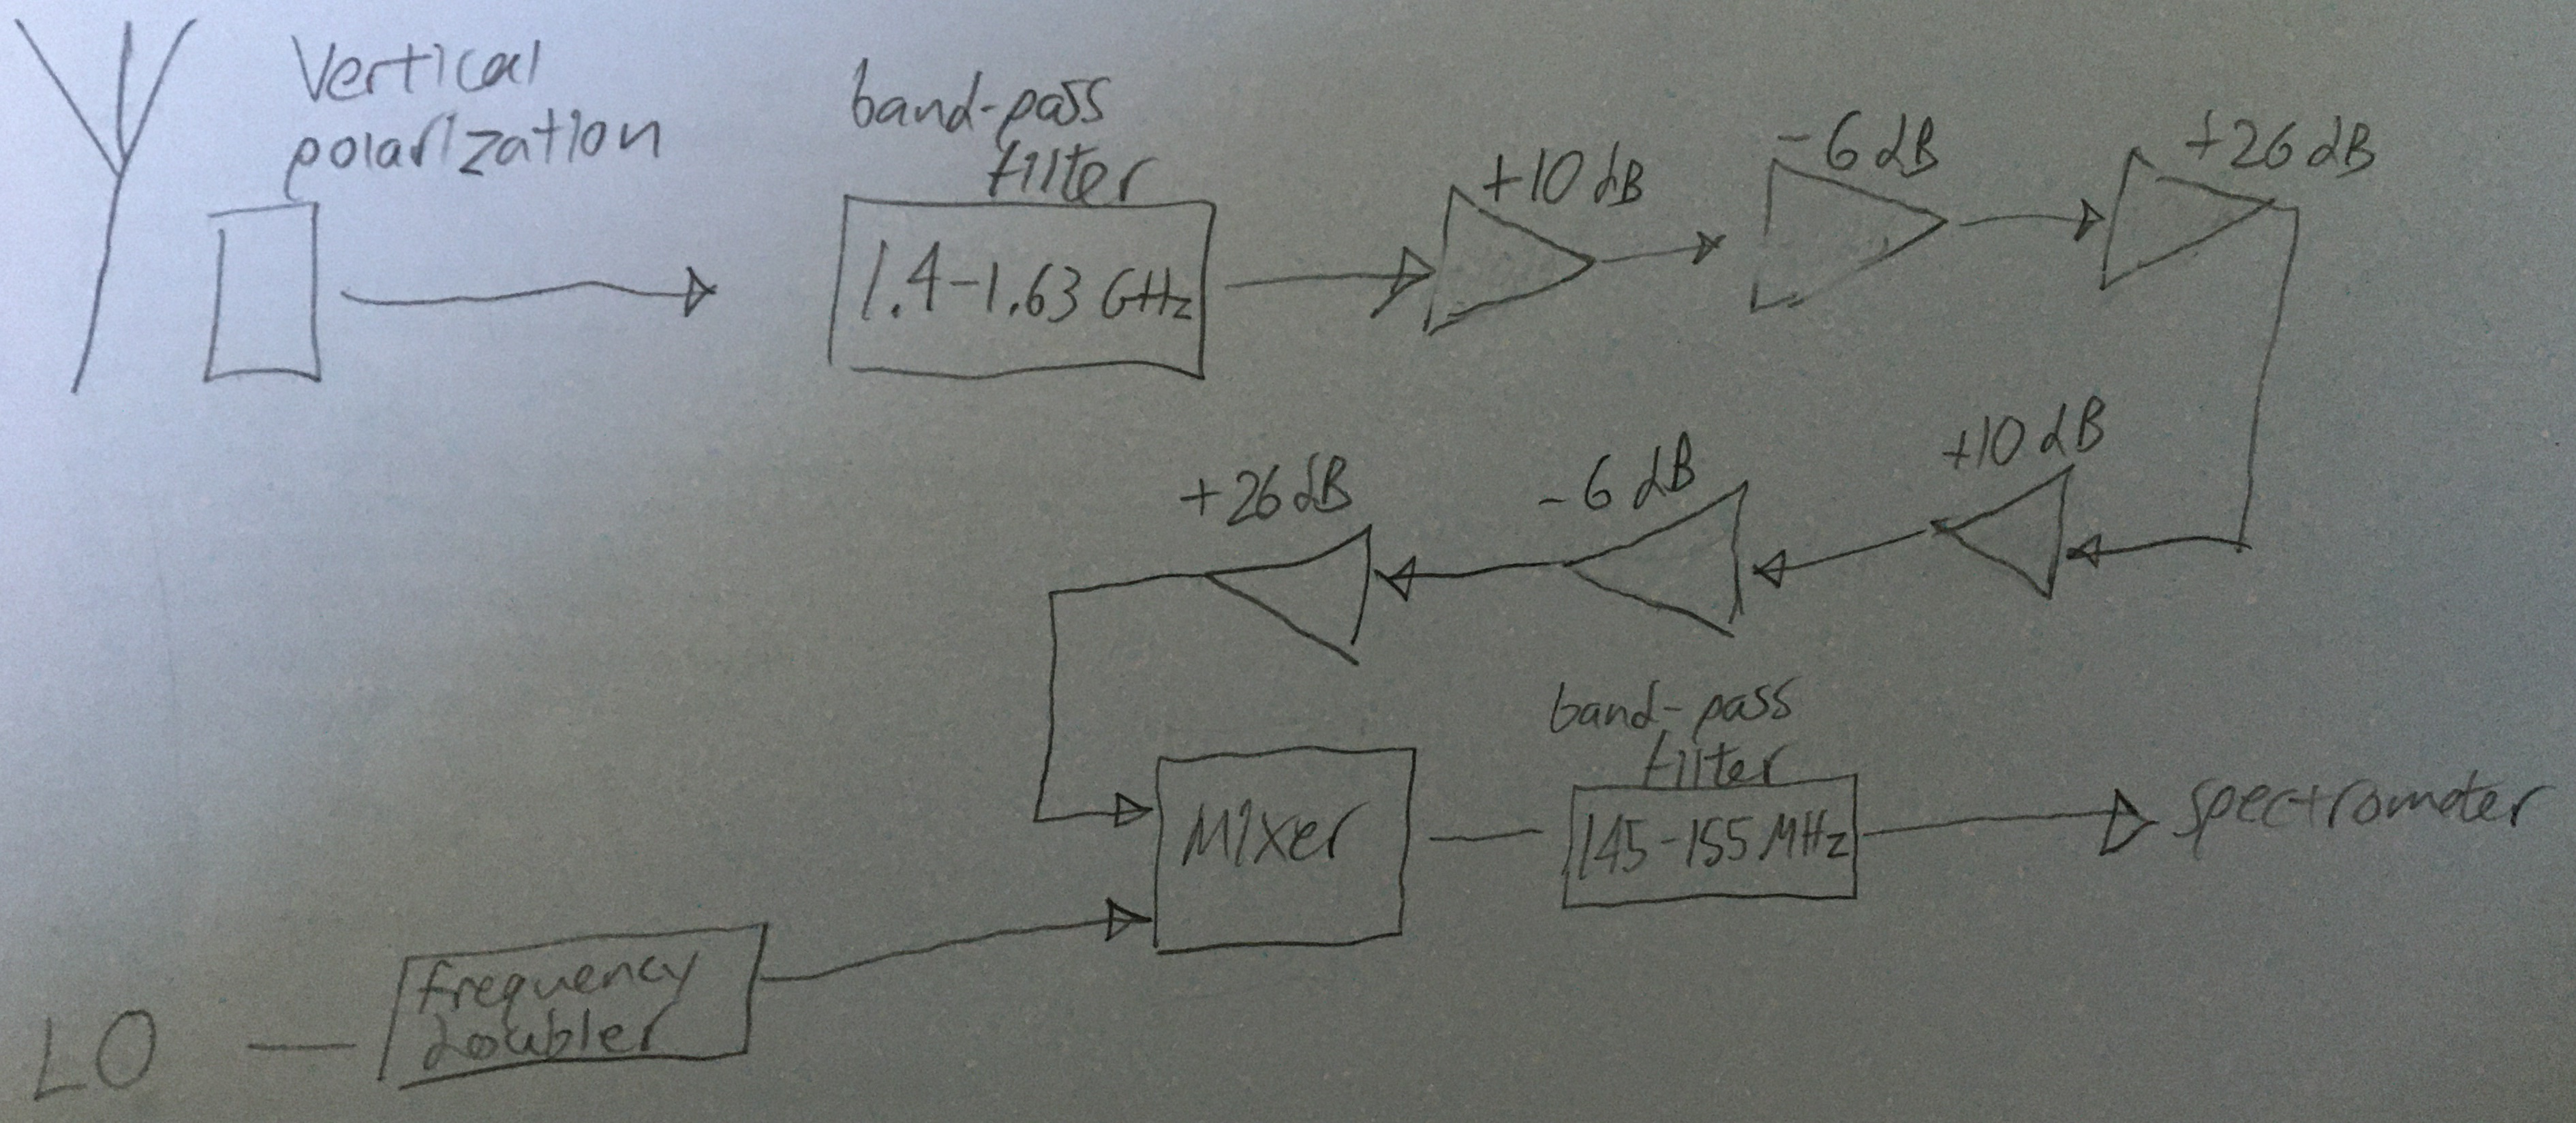
\includegraphics[width=.9\linewidth]{sig_chain}
	\caption{This is a simplification of the Leuschner signal chain, where the horizontal polarization has been ignored (we do not use those data in this report). Furthermore, we abstract-away the clock rate of the ROACH and the various stages of digitization. For our `on' LO frequency of 1270 MHz, the output spectra cover a frequency range 1415 to 1425 MHz.}
	\label{fig:sig_chain}
\end{figure}

The initial band-pass filter ranges from 1.4 to 1.63 GHz. There is a down-converter that mixes this filtered signal with the signal from the local oscillator LO. This leads to a new frequency band (intermediate frequency IF) of 130 MHz to 360 MHz. Since we are using a real-valued mixer, we apply a band-pass filter to eliminate the sum frequencies. This filter is centered at 150 MHz and has a bandwidth of 10 MHz. Consequently, we expect the following frequency range in our outputs (which take the form of spectra in .fits files): a 10 MHz wide range beginning at 145 MHz IF (which maps to 1.415 GHz RF) and ending at 155 MHz IF (which maps to 1.425 GHz RF).

Before we analyze these results, we need to combine each pair of four averaged spectra into a single calibrated spectrum which comprehensively describes our observations for a single galactic coordinate pair. We want to change our local oscillator frequency (as indicated in equation \ref{eq:line_shape}) between two values. This allows us to, via the mixer, adjust where the HI line appears in our spectra. We thereby create `on' (LO at 1270 MHz) and `off' (LO at 1268 MHz) spectra. Our `off' frequency, 1268 MHz, leads to an output range of 1.417 to 1.419 GHz. 

The gain, G (indicated in equation \ref{eq:line_gain}), is calculated with an additional spectrum ($cal$) that we deliberately contaminate with thermal noise. We do this by activating a noise diode wired close to the Leuschner dish receiver. For the vertical-polarization receiver (with which we are exclusively concerned here), the noise diode was independently estimated to contribute about 80 Kelvins. For our `cold' spectrum, we simply use the spectrum measured for the same galactic coordinates but without the noise diode enabled. We control for any time-dependent environmental inconsistencies by taking these two spectra consecutively.

We sample at 24 MHz (we keep 1/32 of the samples from the 768 MHz clock). We have a 12MHz Nyquist bandwidth, and we are operating in the twelfth Nyquist window. To protect our results from noise, we record 10 spectra for each case (on spectrum with noise diode, on spectrum without, off spectrum with noise diode, off spectrum without) and independently average them. Figure \ref{fig:cal_ex}, in our observations section, is an example of a fully calibrated spectrum which shows a sort of HI mirroring effect (a direct consequence of dividing the on and off spectra) as well as a y-axis that is physically meaningful due to this procedure.

\section{Observations}

\begin{figure}
	\centering
	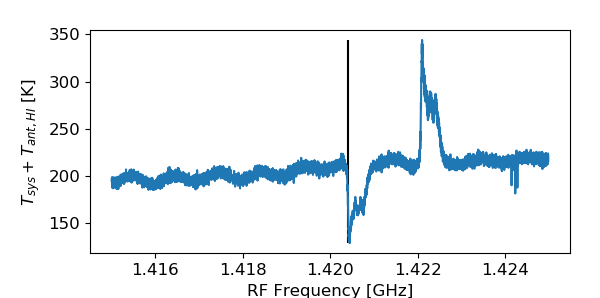
\includegraphics[width=.8\linewidth]{cal_ex_80_deg}
	\caption{This is an example of a fully calibrated spectrum ($\ell = 80^\circ$), for which we have created 260. There is a black vertical line indicating the location of the 21 cm HI line at rest (1420.405751786 MHz at rest). Despite the forty spectra used to produce a single spectrum of this kind, there remain clear limitations to the utility. There is a clear sinusoidal trend (with a sloped baseline) as well as systematics spikes (here visible at 1.424 GHz) which persist across spectra. Our intensity maximizer function is generally resistant to these annoyances due to the comparatively high signal to noise ratio of our setup. Nevertheless, there do exist some exceptions, as our later plots potentially feature.}
	\label{fig:cal_ex}
\end{figure}

\quad \quad By maximizing the brightness temperature for the fully calibrated spectrum (consider how the shape of figure \ref{fig:cal_ex} would be friendly to a primitive maximization algorithm) of every galactic longitude on our range, we are able to produce a single plot which represents an overview of our data for this project. Figure \ref{fig:Dopp_collection} is close to what we would consider our image $T_A(\ell, V_{LSR})$ except that the graph is not colored to reflect varying brightness temperatures at the different angles. However, on its own, the figure does reflect the peculiarity of the various gas clouds in that the plot does not always appear to follow consistent patterns.

% This plot is simply a way of concisely representing the 260 spectra we collected over the interval $\ell \in [-9, 250]$ degrees (one-degree spacings).
\begin{figure}
	\centering
	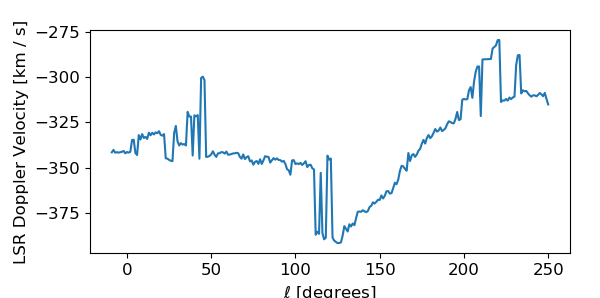
\includegraphics[width=.8\linewidth]{Doppler_collection}
	\caption{We take the peak intensity of each spectrum to represent the shifted HI line for that galactic longitude.  Observe that, for our tangent-point considerations ($\ell \in [0, 90]$), we have an initial region featuring wild fluctuations followed by a relatively flat region for the second half of the angles. While this could represent physical realities, this seeming discontinuity of the derivative could also be a consequence of the primitive intensity-maximizing function, or it could be a consequence of pointing the telescope at angles close to mechanical boundaries.}
	\label{fig:Dopp_collection}
\end{figure}

%\textcolor{red}{This is $almost$ the image $T_A(\ell, V_\text{LSR})$; we need the brightness temperature associated with each Doppler velocity, then we can color this.}

Additionally, we may more quantitatively explore the idea pursued in the illustration for figure \ref{fig:ell_vs_r}. Figure \ref{fig:TP_disp} represents a dispersion of lines relating linear velocity to the distance from the galactic center. We create this visualization by treating radial distance and galactic longitude as parameters essentially independent but for the constraint that $R_\text{min} = R_\odot \sin \ell$ and $R_\text{max} = R_\odot$ (G.L. Verschuur and K. I. Kellermann, 1983). This particular distribution appears highly symmetric, which may at first counter worries as to the rigor of a tangent-point approach.

\begin{figure}
	\centering
	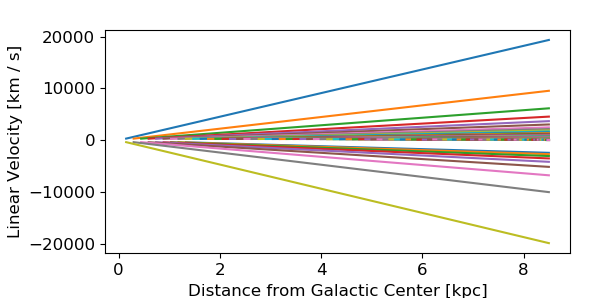
\includegraphics[width=.8\linewidth]{tangentPoint_dispersion}
	\caption{This is an overplot of all 90 possible velocity curves. Specifically, when we treat the solar circle of the galaxy, we know that for each $\ell$, $R$ can take on a maximum value of $R_\odot$ (the radius of the solar circle) and a minimum value of $R_\odot \sin \ell$. The tangent-point method mandates the usage of $R_\text{min}$, but we here demonstrate how that method necessitates the collapse of line segments into points.}
	\label{fig:TP_disp}
\end{figure}

However, since the tangent-point method is applied exclusively to the range $\ell \in (0^\circ, 90^\circ]$, a more relevant comparison is offered in figure \ref{fig:TP_sel_disp}. Selecting the minimum value for radial distance seems more natural as we approach ninety degrees (the arc length vanishes and we are treating one value for radius anyway). However, as we approach the other end, the arc lengths begin to explode.

\begin{figure}
	\centering
	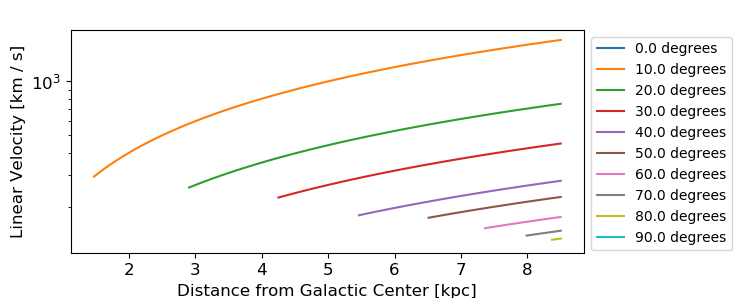
\includegraphics[width=.9\linewidth]{tangentPoint_selected_dispersions}
	\caption{Here we are essentially representing similar information to that of figure \ref{fig:TP_disp}. We use a semilog vertical axis to verify that there is one consistently-varying multiplicative offset ($\frac{1}{\sin \ell}$) as we examine different galactic longitudes. This plot also agrees with our expectation that our two boundary cases are meaningless: $\ell = 0^\circ$ approaches an infinite linear velocity and $\ell = 90^\circ$ corresponds to a velocity curve for which the minimum and maximum radii are the same (an infinitesimal segment).}
	\label{fig:TP_sel_disp}
\end{figure}

Ten degrees is still far from our lower bound of zero, but we can see here that the single galactic longitude spans a linear velocity of around an order of magnitude. Furthermore, we need radius anyway for our classical mass considerations (refer to equation \ref{eq:mass}), and the problem is more concerning for that (we nearly span the full range of the solar circle). With a square term on velocity and a first-order radius term, we can expect a range of values which span nearly three orders of magnitude on mass. This author lacks sufficient understanding of the tangent-point method to make conclusions about its accuracy, which means that this situation is neither a problem to be ignored nor, necessarily, a problem to which to draw academic attention.

\section{Analysis}

\begin{figure}
	\centering
	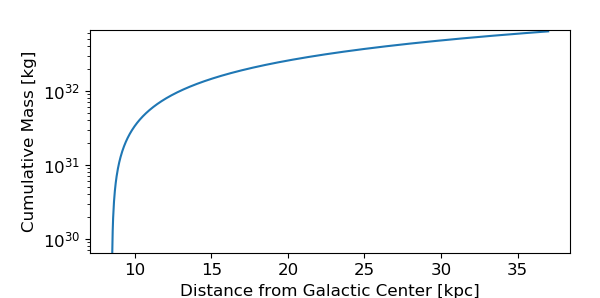
\includegraphics[width=.8\linewidth]{outer_mass_distro}
	\caption{This is a cumulative mass distribution for radii larger than that of the solar circle. The plot begins with a mass of zero because we subtract-off whatever the function calculates for radii smaller than that of the solar circle; we know the calculations to be erroneous for the smaller radii because we are applying different calculation methods. Observe that the rate of increase of mass drops off rather steeply. We hope for this to be the case as the galaxy thins out toward its edges and is most dense at smaller radii. However, the transition is rather jarring to be ocurring as far out as the Sun. It may point to a deficiency in the mass approximation near $R_\odot$.}
	\label{fig:outer_mass_distro}
\end{figure}

\quad \quad If we take the $V(R) \approx 220$ km/s for $R > R_\odot \approx 8.5$ kpc, we may apply equation \ref{eq:mass} out to radius of the Milky Way, estimated to be about 18.5 kpc (M. L\'{o}pez-Corredoira et al, 2018). This corresponds to the ideal cumulative mass plot, figure \ref{fig:outer_mass_distro}. The final mass, for the range exclusively defined as the outer region of the Milky Way, rests at $2.23808 \times 10^{32}$ kg (about one hundred solar masses).

\begin{figure}
	\centering
	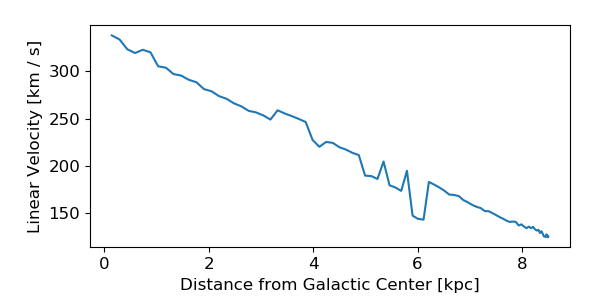
\includegraphics[width=.8\linewidth]{inner_vel_distro}
	\caption{This is a plot of galactic rotation velocities by radius, calculated using the tangent-point method. If we approximated the galactic plane as a rigid disk, we would expect the velocity to increase with greater radius (as the same angular distance must be covered in the same amount of time at a greater radius). While this line does not disqualify a spiral, we might initially expect a spiral shape to come from $similar$ linear velocities manifesting as curved arms at greater radii. It is not clear if the fall-off of gravitational influence would agree with this model.}
	\label{fig:inner_vel_distro}
\end{figure}

To examine the mass $in$side the solar circle, we have to use a different approach: the tangent-point method described in the introduction. Figure \ref{fig:inner_vel_distro} is created with 89 points. Each point has an x coordinate corresponding to the minimum radial distance $R_\text{min} = R_\odot \sin \ell$. We then plug that $R_\text{min}$ into equation \ref{eq:vel_curve} and combine our observations for Doppler velocity (corrected for the local standard of rest frame). We observe a linear and almost monotonic decrease for the entire range of the solar circle, which may be consistent with the spiral model distribution of linear velocities.

\begin{figure}
	\centering
	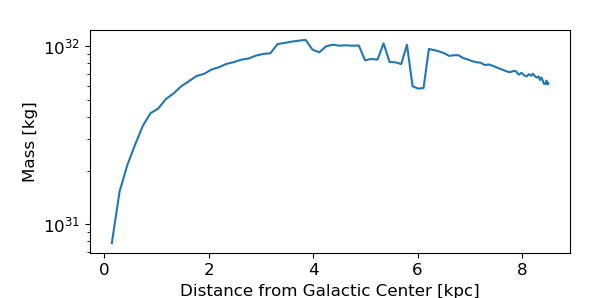
\includegraphics[width=.8\linewidth]{inner_mass_distro}
	\caption{This is a semilog plot of interstellar cloud mass versus radius. The calculation rests conceptually on a cumulative distribution function, so we may immediately spot imperfections in the data. Specifically, after about 3 kpc, the data do not leveling off consistently. Instead, the mass response fluctuates and then slowly declines. However, the initial rise does fit with our expectation of a general decrease in density as we move outward from the center.}
	\label{fig:inner_mass_distro}
\end{figure}

Now, figure \ref{fig:inner_vel_distro} only charts the velocity calculations. We are here interested in the quantities of mass in the solar circle, so we apply equation \ref{eq:mass} to these results to get figure \ref{fig:inner_mass_distro}. We expect the the result to be a cumulative distribution function, so the decrease toward the end is disconcerting. This results in a maximum spread of about 48\% in the final result. We estimate the gaseous mass inside the solar circle to be $(8.16075 \pm .19450) \times 10^{31}$ kg. This is only about 40 solar masses, the error is not large enough to really escape suspicion. We expect the milky way galaxy to be forming new stars at a very high rate, but there is simply not enough mass in this calculation to justify any such concept.

Furthermore, this is about one order of magnitude smaller than our analogous result for the outer milky way. We expect a decreasing density function with increasing radius, so we doubt this result for a second reason.

Finally, we can estimate the mass of the super-massive black hole at the center of the milky way if we use the Doppler velocity for our closest angle ($\ell = 1^\circ$) and combine equations \ref{eq:vel_curve} and \ref{eq:mass} and integrate over radii from the galactic center out to a single light-year. Modern estimates of the radius of the active galactic nucleus put it at about $4.4 \times 10^{7}$ km in radius (Doelemean et al, 2008). By comparison, a light year is six orders of magnitude larger than the estimated radius of the black hole.

With a simple integration over the black hole radius, we get a mass of approximately $7.52497 \times 10^{22}$ kg. This is eight orders of magnitude below the mass of the sun, so we immediately know the result to be spurious. Anyway, the independent mass is published to be about 6 orders of magnitude greater than the mass of the sun (Doelemean et al, 2008).

Error is very difficult to consider here because the radius would otherwise be chosen quite arbitrarily. Truly, we are observing the movement of gaseous clouds $around$ the black hole, so one would be tempted to correct this underestimation by expanding the effective radius. However, it is not clear what boundary to set. What qualifies as `very close' to the black? If we expand to one light year (which may indeed be considered very close for a supermassive black hole), the calculated mass of course increases by six orders of magnitude.

To reverse-engineer the published result using this approach, we would have to define `very close' as one hundred million light-years. This is already orders of magnitude larger than the radius of the Milky Way galaxy. Therefore, without a satisfactory numerical error, we may still conclude that something in this estimation was fundamentally flawed, for we lack even a distantly-correct figure.

\section{Conclusions}

\quad \quad In summary, the mass considerations were bad.

\section{Acknowledgments}

\quad \quad Mehdi developed column density examples for calculating the mass, as well as some routines for parsing .fits data. Rebecca developed filtering examples for subtracting-off the sytematics spikes, curved baseline, and sinusoidal pattern shown in figure \ref{fig:cal_ex}. I wrote most of the code to adapt the old tracking script to this new project, and took several sets of data to resolve localized errors.

Theory and background provided by Aaron Parsons. ``LAB 4: Mapping the Galactic HI Line.'' Updated April 2020.

% The following is a lorem ipsum. We want
	% tangent-point resource recommended by Rebecca
	% my source for the radius of the galactic black hole
	% lab 2, for most of the gain and line shape stuff. Should I also cite myself?

\begin{thebibliography}{4}

\bibitem{doeleman}
S. Doeleman et al.
\textit{Event-horizon-scale structure in the supermassive black hole candidate at that Galactic Centre}.
Nature, 455(7209):78–80, 2008.

\bibitem{me}
L. Finkbeiner.
\textit{Lab 2}.
2020.

\bibitem{lopez}
M. L\'{o}pez-Corredoira, C. Allende Prieto, F. Garzón, H. Wang, C. Liu and L. Deng.
\textit{Disk stars in the Milky Way detected beyond 25 kpc from its center}.
Astronomy \& Astrophysics 612: L8, 2018.

\bibitem{verschuur} 
G.L. Verschuur and K. I. Kellermann. 
\textit{Galactic and Extragalactic Radio Astronomy}. 
Springer-Verlag, 1983.

\end{thebibliography}

\end{document}
